\documentclass{article}
\usepackage[utf8]{inputenc}
\usepackage{geometry}
\usepackage[T1]{fontenc}
\usepackage{amsfonts}
\usepackage{graphicx}
\usepackage{float}
\usepackage{hyperref}
\usepackage[sorting=none]{biblatex}
\usepackage{fancyhdr}
\usepackage{multicol}
\addbibresource{ref.bib}
\setlength{\columnsep}{40pt}
\setlength{\voffset}{0.7cm}
\setlength{\headsep}{40pt}
\geometry{legalpaper, portrait, margin=2cm}


% Title page
\title{Essay title\\\Large{Machine Learning, Advanced Course/DD2434/mladv24}}
\author{Aurhor \\ KTH Royal Institute of Technology\\ School of Engineering Sciences in Chemistry, Biotechnology and Health}
\date{\today}

% Header and footer
\pagestyle{fancy}
\fancyhead{}
\fancyhead[L]{\textbf{Machine Learning, Advanced Course}\\\textbf{DD2434}}
\fancyhead[R]{\textbf{Andrea Stanziale, Leonardo Lüder}\\ stanziale@kth.se, luder@kth.se}
\fancyfoot{}
\begin{document}

\maketitle
\thispagestyle{fancy}
\clearpage
\tableofcontents
\thispagestyle{fancy}

\clearpage
% Begin page numbers
\fancyfoot[C]{\thepage}
\pagenumbering{arabic}
\begin{multicols}{2}

    \section*{1.1}

    \section*{1.2}

    \subsection*{1.2.7}
    We implement a function that generates a dataset of $N$ points in the plane, where each point is drawn from a normal distribution with mean $\mu$ and precision $\tau$. For reproducability we set the seed of the random number generator to 0. We generate datasets for $N = 10, 100, 1000$ and plot the generated values as histograms, which results in figure \autoref{fig:histograms_datasets}. 

    
    \begin{figure}[H]
        \centering
        \begin{minipage}{0.32\textwidth}
            \centering
            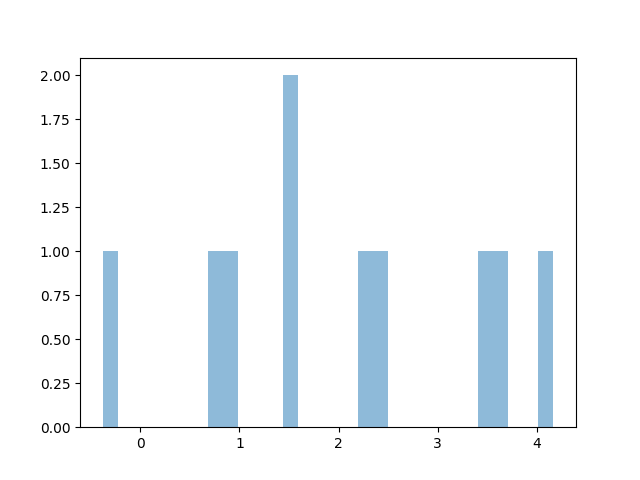
\includegraphics[width=\textwidth]{figures/1.2/dataset_1.png}
            \caption{N=10}
        \end{minipage}
        \hfill
        \begin{minipage}{0.32\textwidth}
            \centering
            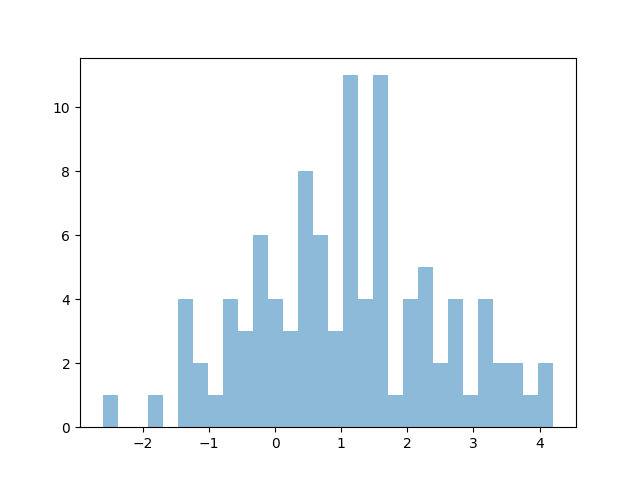
\includegraphics[width=\textwidth]{figures/1.2/dataset_2.png}
            \caption{N=100}
        \end{minipage}
        \hfill
        \begin{minipage}{0.32\textwidth}
            \centering
            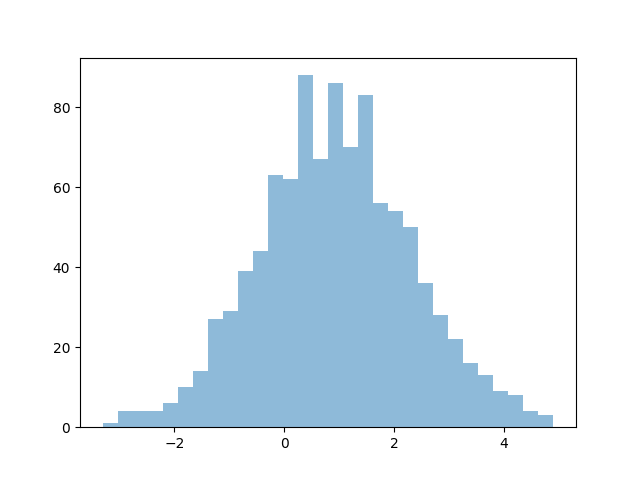
\includegraphics[width=\textwidth]{figures/1.2/dataset_3.png}
            \caption{N=1000}
        \end{minipage}
        \caption{Histograms of generated datasets}\label{fig:histograms_datasets}
    \end{figure}

    We see that the more datapoints we have the more the histogram resembles a normal distribution which is as expected.


\end{multicols}
\clearpage
\addcontentsline{toc}{section}{References}
\printbibliography{}

\end{document}
